\subsection{Retrieving a known structure}
\subsubsection*{Test networks and evaluation techniques}

We used two well-known network structures. The first, \textsc{asia}, was introduced by \cite{Lau88} (cf figure~\ref{orig}.a).
All its nodes are binary nodes. We can notice that concerning the edge between $A$ et $T$, the  \emph{a priori} probability of $A$ is small, and the influence of $A$ on $T$ is weak.
The second network we use is \textsc{insurance} with $27$ nodes (cf figure \ref{orig}.b) and is available in \cite{BNR97}.

Data generation has been performed for different sample sizes in order to test the influence of this size over the results of the various structure learning methods.
To generate a sample, we draw the parent node values randomly and choose the son node values according to the Bayesian network parameters.
\vspace*{-\baselineskip}

\begin{figure}[!ht]
\centering\begin{tabular}{ll}\hspace*{1cm}
\begin{minipage}{6cm}
\hspace*{-195pt}\vspace*{-175pt}
%{\xymatrix@C=4pt @R=9pt{*+[F]{A} \ar[d] & & & *+[F]{S} \ar[dl] \ar[dr] \\ *+[F]{T} \ar[dr] &  & *+[F]{L} \ar[dl] &  & *+[F]{B} \ar[ddll] \\ & *+[F]{E} \ar[dl] \ar[dr] \\ *+[F]{X} & & *+[F]{D}}} 
 \includegraphics[width=55mm, height=52mm]{fig/asia2}
\end{minipage} & %\hspace*{2cm} &
\hspace*{-240pt}
\begin{minipage}{6cm}
 \includegraphics[width=110mm, height=110mm]{fig/insurance}
\end{minipage}\\
\hspace*{-80pt}(a) & \hspace*{-80pt} (b)
\end{tabular}
\caption{Original networks : (a) \textsc{asia} and (b) \textsc{insurance}}
\label{orig}
\end{figure}

\begin{table}[!p]
\vspace*{-\baselineskip}
\hspace*{-5mm}
%\begin{tabular}{r@{}c@{\,}c@{\,}c@{\,}c@{\,}c@{}c@{}c}
%\begin{tabular}{r@{}p{2.05cm}@{\,}p{2.05cm}@{\,}p{2.05cm}@{\,}p{2.05cm}@{\,}p{2.05cm}@{}p{2.05cm}@{}p{2.05cm}}
\begin{tabular}{r@{}p{2.0cm}@{}p{2.0cm}@{}p{2.0cm}@{}p{2.0cm}@{}p{2.0cm}@{}p{2.0cm}@{}p{2.0cm}}
 & \textbf{~~~~~250} & \textbf{~~~~~500} & \textbf{~~~~1000} & \textbf{~~~~2000} & \textbf{~~~~5000} & \textbf{~~~10000} & \textbf{~~~15000} \\
\textsc{mwst~} &
\includegraphics[width=20.3mm, height=14.25mm]{fig/11-Sep-2003-14-42-00-dag-asia250-MSWT-RES} &
\includegraphics[width=20.3mm, height=14.25mm]{fig/11-Aug-2003-13-48-14-dag-asia500-MSWT-RES} &
\includegraphics[width=20.3mm, height=14.25mm]{fig/19-Feb-2003-16-04-58-dag-asia1000-MSWT-RES} &
\includegraphics[width=20.3mm, height=14.25mm]{fig/19-Feb-2003-16-04-58-dag-asia2000-MSWT-RES} &
\includegraphics[width=20.3mm, height=14.25mm]{fig/19-Feb-2003-16-04-58-dag-asia5000-MSWT-RES} &
\includegraphics[width=20.3mm, height=14.25mm]{fig/19-Feb-2003-16-04-58-dag-asia10000-MSWT-RES} &
\includegraphics[width=20.3mm, height=14.25mm]{fig/19-Feb-2003-16-04-58-dag-asia15000-MSWT-RES} \\
& 9;-68837 & 10;-69235 & 8;-68772 & 6;-68704 & 7;-68704 & 3;-68694 & 3; -68694 \\
\textsc{pc~} &
\includegraphics[width=20.3mm, height=14.25mm]{fig/11-Sep-2003-14-27-53-dag-asia250-PC-RES} &
\includegraphics[width=20.3mm, height=14.25mm]{fig/11-Aug-2003-14-06-42-dag-asia500-GES-RES} &
\includegraphics[width=20.3mm, height=14.25mm]{fig/11-Aug-2003-14-06-42-dag-asia1000-GES-RES} &
\includegraphics[width=20.3mm, height=14.25mm]{fig/11-Aug-2003-14-06-42-dag-asia2000-GES-RES} &
\includegraphics[width=20.3mm, height=14.25mm]{fig/11-Aug-2003-14-06-42-dag-asia5000-GES-RES} &
\includegraphics[width=20.3mm, height=14.25mm]{fig/11-Aug-2003-14-06-42-dag-asia10000-GES-RES} &
\includegraphics[width=20.3mm, height=14.25mm]{fig/11-Aug-2003-14-06-42-dag-asia15000-GES-RES} \\
& 8;-55765 & 7;-66374 & 6;-61536 & 7;-56386 & 6;-63967 & 5;-63959 & 6;-70154\\
\textsc{bn-pc~} &
\includegraphics[width=20.3mm, height=14.25mm]{fig/11-Sep-2003-14-37-15-dag-asia250-BNPC-RES} &
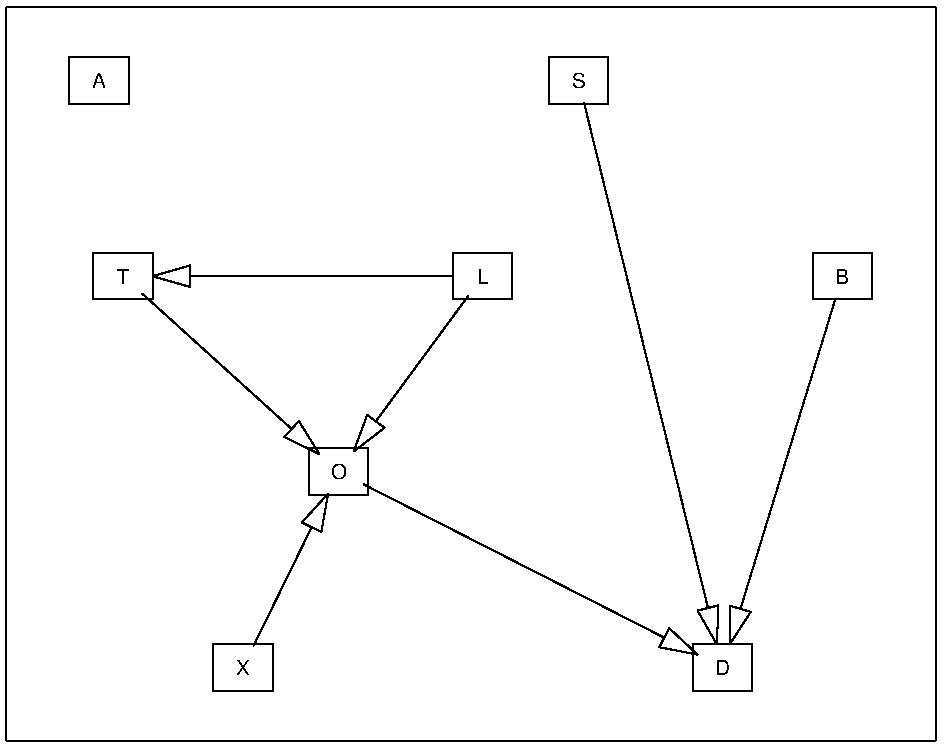
\includegraphics[width=20.3mm, height=14.25mm]{fig/12-Aug-2003-16-26-12-dag-asia500-BNPC-RES} &
\includegraphics[width=20.3mm, height=14.25mm]{fig/12-Aug-2003-16-26-12-dag-asia1000-BNPC-RES} &
\includegraphics[width=20.3mm, height=14.25mm]{fig/12-Aug-2003-16-26-12-dag-asia2000-BNPC-RES} &
\includegraphics[width=20.3mm, height=14.25mm]{fig/12-Aug-2003-16-34-51-dag-asia5000-BNPC-RES} &
\includegraphics[width=20.3mm, height=14.25mm]{fig/12-Aug-2003-16-41-03-dag-asia10000-BNPC-RES} &
\includegraphics[width=20.3mm, height=14.25mm]{fig/12-Aug-2003-16-41-03-dag-asia15000-BNPC-RES} \\
& 11;-67825 & 6;-73885 & 6;-72529 & 6;-72529 & 7;-73141 & 6;-69046 & 6;-69370\\
\textsc{k2~} &
\includegraphics[width=20.3mm, height=14.25mm]{fig/11-Sep-2003-14-28-11-dag-asia250-K2-RES} &
\includegraphics[width=20.3mm, height=14.25mm]{fig/11-Aug-2003-14-51-45-dag-asia500-K2-RES} &
\includegraphics[width=20.3mm, height=14.25mm]{fig/11-Mar-2003-18-40-53-dag-asia1000-K2-RES} &
\includegraphics[width=20.3mm, height=14.25mm]{fig/11-Mar-2003-18-40-53-dag-asia2000-K2-RES} &
\includegraphics[width=20.3mm, height=14.25mm]{fig/11-Mar-2003-18-40-53-dag-asia5000-K2-RES} &
\includegraphics[width=20.3mm, height=14.25mm]{fig/11-Mar-2003-18-40-53-dag-asia10000-K2-RES} &
\includegraphics[width=20.3mm, height=14.25mm]{fig/11-Mar-2003-18-40-53-dag-asia15000-K2-RES} \\
& 8;-68141 & 7;-67150 & 6;-67152 & 6;-67147 & 6;-67106 & 6;-67106 & 6;-67106\\
\textsc{k2(2)~} &
\includegraphics[width=20.3mm, height=14.25mm]{fig/11-Sep-2003-14-47-35-dag-asia250-K2-RES} &
\includegraphics[width=20.3mm, height=14.25mm]{fig/11-Aug-2003-14-59-43-dag-asia500-K2-RES} &
\includegraphics[width=20.3mm, height=14.25mm]{fig/11-Mar-2003-18-46-18-dag-asia1000-K2-RES} &
\includegraphics[width=20.3mm, height=14.25mm]{fig/11-Mar-2003-18-46-18-dag-asia2000-K2-RES} &
\includegraphics[width=20.3mm, height=14.25mm]{fig/11-Mar-2003-18-46-18-dag-asia5000-K2-RES} &
\includegraphics[width=20.3mm, height=14.25mm]{fig/11-Mar-2003-18-46-18-dag-asia10000-K2-RES} &
\includegraphics[width=20.3mm, height=14.25mm]{fig/11-Mar-2003-18-46-18-dag-asia15000-K2-RES} \\
& 11;-68643 & 11;-68089 & 11;-67221 & 10;-67216 & 9;-67129 & 9;-67129 & 9;-67129\\
\textsc{k2+t~} &
\includegraphics[width=20.3mm, height=14.25mm]{fig/11-Sep-2003-14-28-11-dag-asia250-K2+MSWT-RES} &
\includegraphics[width=20.3mm, height=14.25mm]{fig/11-Aug-2003-14-51-45-dag-asia500-K2+MSWT-RES} &
\includegraphics[width=20.3mm, height=14.25mm]{fig/11-Mar-2003-18-40-53-dag-asia1000-K2+MSWT-RES} &
\includegraphics[width=20.3mm, height=14.25mm]{fig/11-Mar-2003-18-40-53-dag-asia2000-K2+MSWT-RES} &
\includegraphics[width=20.3mm, height=14.25mm]{fig/11-Mar-2003-18-40-53-dag-asia5000-K2+MSWT-RES} &
\includegraphics[width=20.3mm, height=14.25mm]{fig/11-Mar-2003-18-40-53-dag-asia10000-K2+MSWT-RES} &
\includegraphics[width=20.3mm, height=14.25mm]{fig/11-Mar-2003-18-40-53-dag-asia15000-K2+MSWT-RES} \\
& 10;-68100 & 8;-68418 & 9;-67185 & 8;-67317 & 8;-67236 & 10;-67132 & 10;-67132\\
\textsc{k2-t~} &
\includegraphics[width=20.3mm, height=14.25mm]{fig/11-Sep-2003-14-47-35-dag-asia250-K2-MSWT-RES} &
\includegraphics[width=20.3mm, height=14.25mm]{fig/11-Aug-2003-14-59-43-dag-asia500-K2-MSWT-RES} &
\includegraphics[width=20.3mm, height=14.25mm]{fig/11-Mar-2003-18-46-18-dag-asia1000-K2-MSWT-RES} &
\includegraphics[width=20.3mm, height=14.25mm]{fig/11-Mar-2003-18-46-18-dag-asia2000-K2-MSWT-RES} &
\includegraphics[width=20.3mm, height=14.25mm]{fig/11-Mar-2003-18-46-18-dag-asia5000-K2-MSWT-RES} &
\includegraphics[width=20.3mm, height=14.25mm]{fig/11-Mar-2003-18-46-18-dag-asia10000-K2-MSWT-RES} &
\includegraphics[width=20.3mm, height=14.25mm]{fig/11-Mar-2003-18-46-18-dag-asia15000-K2-MSWT-RES} \\
& 7;-68097 & 6;-67099 & 6;-67112 & 7;-67105 & 6;-67091 & 5;-67091 & 5;-67091\\
\textsc{gs-0~} &
\includegraphics[width=20.3mm, height=14.25mm]{fig/11-Sep-2003-14-39-38-dag-asia250-GS-RES} &
\includegraphics[width=20.3mm, height=14.25mm]{fig/11-Aug-2003-15-08-57-dag-asia500-GS-RES} &
\includegraphics[width=20.3mm, height=14.25mm]{fig/26-Feb-2003-16-33-13-dag-asia1000-GS-RES} &
\includegraphics[width=20.3mm, height=14.25mm]{fig/26-Feb-2003-16-33-13-dag-asia2000-GS-RES} &
\includegraphics[width=20.3mm, height=14.25mm]{fig/26-Feb-2003-16-33-13-dag-asia5000-GS-RES} &
\includegraphics[width=20.3mm, height=14.25mm]{fig/26-Feb-2003-16-33-13-dag-asia10000-GS-RES} &
\includegraphics[width=20.3mm, height=14.25mm]{fig/26-Feb-2003-16-33-13-dag-asia15000-GS-RES} \\
& 4;-67961 & 9;-68081 & 2;-67093 & 5;-67096 & 7;-67128 & 9;-67132 & 8;-67104 \\
\textsc{gs+t~} &
\includegraphics[width=20.3mm, height=14.25mm]{fig/11-Sep-2003-14-39-38-dag-asia250-GS-MSWT-RES} &
\includegraphics[width=20.3mm, height=14.25mm]{fig/11-Aug-2003-15-08-57-dag-asia500-GS-MSWT-RES} &
\includegraphics[width=20.3mm, height=14.25mm]{fig/26-Feb-2003-16-33-13-dag-asia1000-GS-MSWT-RES} &
\includegraphics[width=20.3mm, height=14.25mm]{fig/26-Feb-2003-16-33-13-dag-asia2000-GS-MSWT-RES} &
\includegraphics[width=20.3mm, height=14.25mm]{fig/26-Feb-2003-16-33-13-dag-asia5000-GS-MSWT-RES} &
\includegraphics[width=20.3mm, height=14.25mm]{fig/26-Feb-2003-16-33-13-dag-asia10000-GS-MSWT-RES} &
\colorbox{Ocase}{\includegraphics[width=20.3mm, height=14.25mm]{fig/26-Feb-2003-16-33-13-dag-asia15000-GS-MSWT-RES}} \\
& 9;-68096 & 6;-68415 & 2;-67093 & 7;-67262 & 2;-67093 & 2;-67093 & \colorbox{Ocase}{1;-67086~~~} \\
\textsc{ges~} &
\includegraphics[width=20.3mm, height=14.25mm]{fig/11-Sep-2003-14-43-10-dag-asia250-GES-RES} &
\includegraphics[width=20.3mm, height=14.25mm]{fig/11-Aug-2003-13-36-32-dag-asia500-GES-RES} &
\includegraphics[width=20.3mm, height=14.25mm]{fig/28-Jul-2003-17-49-38-dag-asia1000-GES-RES} &
\includegraphics[width=20.3mm, height=14.25mm]{fig/28-Jul-2003-17-49-38-dag-asia2000-GES-RES} &
\colorbox{Ocase}{\includegraphics[width=20.3mm, height=14.25mm]{fig/28-Jul-2003-17-49-38-dag-asia5000-GES-RES}} &
\colorbox{Ocase}{\includegraphics[width=20.3mm, height=14.25mm]{fig/28-Jul-2003-17-49-38-dag-asia10000-GES-RES}} &
\colorbox{Ocase}{\includegraphics[width=20.3mm, height=14.25mm]{fig/28-Jul-2003-17-49-38-dag-asia15000-GES-RES}} \\
& 4;-68093 & 6;-68415 & 5;-67117 & 2;-67094 & \colorbox{Ocase}{0;-67086~~~} & \colorbox{Ocase}{0;-67086~~~} & \colorbox{Ocase}{0;-67086~~~} \\
% \textsc{sem~} &
% \includegraphics[width=20.3mm, height=14.25mm]{fig/11-Sep-2003-15-01-29-dag-asia250-SEM-RES} &
% \includegraphics[width=20.3mm, height=14.25mm]{fig/11-Aug-2003-15-18-25-dag-asia500-SEM-RES} &
% \includegraphics[width=20.3mm, height=14.25mm]{fig/12-Mar-2003-08-44-11-dag-asia1000-SEM-RES} &
% \includegraphics[width=20.3mm, height=14.25mm]{fig/12-Mar-2003-08-44-11-dag-asia2000-SEM-RES} &
% \includegraphics[width=20.3mm, height=14.25mm]{fig/12-Mar-2003-08-44-11-dag-asia5000-SEM-RES} &
% \includegraphics[width=20.3mm, height=14.25mm]{fig/12-Mar-2003-08-44-11-dag-asia10000-SEM-RES} &
% \includegraphics[width=20.3mm, height=14.25mm]{fig/12-Mar-2003-08-44-11-dag-asia15000-SEM-RES} \\
% & 10;-83615 & 9;-81837 & 2;-67093 & 8;-67384 & 4;-67381 & 5;-67108 & 4;-67381 \\
\end{tabular}
\caption{Editing measures, networks and BIC scores obtained with different methods (in row) for several dataset lengths (in column).}
\label{asia}
\end{table}

\begin{table}[!t]
\centering
\begin{tabular}{|@{\,}l@{}|c@{\,}c@{\,}c@{\,}c@{\,}c@{\,}c@{\,}c@{\,}|}\hline
\underline{\large\textsc{\textbf{Insurance}}\normalsize} & 250 & 500 & 1000 & 2000 & 5000 & 10000 & 15000\\\hline
\textsc{mwst} & \,\textbf{37};-3373\, & \,\textbf{34};-3369\, & \,36;-3371\, & \,35;-3369\, & \,34;-3369\, & \,34;-3369\, & \,34;-3369\, \\\hline
\textsc{k2}   & 56,-3258 & 62;-3143 & 60;-3079 & 64;-3095 & 78;-3092 & 82;-3080 & 85;-3085 \\
\textsc{k2(2)}& \textbf{26};-3113 & \textbf{22};-2887 & \textbf{20};-2841 & \textbf{21};-2873 & \textbf{21};-2916 & \textbf{18};-2904 & \textbf{22};-2910 \\
\textsc{k2+t} & 42;-3207 & 40;-3009 & 42;-3089 & 44;-2980 & 47;-2987 & 51;-2986 & 54;-2996 \\
\textsc{k2-t} & 55;-3298 & 57;-3075 & 57;-3066 & 65;-3007 & 70;-2975 & 72;-2968 & 73;-2967 \\\hline
\textsc{mcmc}$^*$ & 50;-3188 & 44;-2967 & 46;-2929 & 40;-2882 & 50;-2905 & 51;-2898 & 54;2892 \\\hline
\textsc{gs}   & \textbf{37};-3228 & 39;-3108 & \textbf{30};-2944 & 33;-2888 & \textbf{29};-2859 & 25;-2837 & 28;-2825 \\
\textsc{gs+t} & 43;-3255 & \textbf{35};-3074 & \textbf{28};-2960 & \textbf{26};-2906 & 33;-2878 & \textbf{19};-2828 & \textbf{21};-2820 \\\hline
\textsc{ges}  & 43;-2910 & 41;-2891 & 39;-2955 & 41;-2898 & 38;-2761 & 38;-2761 & 38;-2752 \\\hline
%\textsc{sem}  & 50;-4431 & 57;-4262 & 61;-4396 & 61;-4092 & 69;-4173 & 63;-4105 & 63;-3978 \\\hline
\end{tabular}
\caption{Editing measures and BIC scores, divided by 100 and rounded, obtained with different methods (in row) for several dataset lengths (in column) ($^*$ As the method MCMC is not deterministic, the results are meaned over five runs).}
\label{resinsur}
\end{table}


\normalsize

In order to compare the results obtained by the different algorithms we tested, we use an 'editing measure' defined by the length of the minimal sequence of operators needed to transform the original graph into the resulting one (operators are edge-insertion, edge-deletion and edge-reversal, note that the edge-reversal is considered as a independent operator and not as the deletion and insertion of the opposite edge).

The BIC score of networks is also precised in a comparative way (computed from additional datasets of $30000$ cases for \textsc{asia} and $20000$ cases for \textsc{insurance}).

\subsubsection*{Results and interpretations}
~\\\textit{Dataset length influence}~\\
Figure \ref{asia} shows us that MWST algorithm appears to be quite insensitive to the length of the dataset.
It always gives a graph close to the original one, although the search space is the tree space which is poorer than the \textsc{dag}s-space .

The PC also gives good results with a  small number of \textit{wrong} edges.

The K2 method is very fast and is frequently used in the literature but presents the drawback of being very sensitive to its initial enumeration order.
Figure \ref{asia} shows the results of K2 on \textsc{asia} data with 2 different orders ("\textsc{elbxasdt}" and "\textsc{taldsxeb}").
We can notice that the results are constant for a given initialization order, but two different initialization orders will lead to very different solutions.
This phenomenon can also be observed in figure \ref{resinsur} with the \textsc{insurance} data sets.

The results given by the BNPC algorithm are good in arc retrieval but do not have great scores.%\footnote{As this method performs statistical tests it can retrieve dependencies that cannot be modelized by a \text{dag} then the last step which consists or orienting edges cannot be performed systematically (maybe this problem is due to our actual implementation).}

The MCMC based method permit to obtain good results whatever the dataset length. In all runs, this method has given similar results from a scoring point of view but there was significant differences among the editing distances.

The GS algorithm is robust to dataset length variation, especially when this algorithm is initialized with \textsc{mwst} tree.

The GES method has given good results whatever the dataset length.
Given an significant amount of data, the networks issued from this method return better scores than those found by a classical greedy search.
But for the more complex \textsc{insurance} network, the results are significantly better as for the scoring function than those obtained with a greedy search in the \textsc{dag}s space but are worse in terms of editing distances.

~\\\textit{Weak dependance recovering}~\\
Most of the tested methods have not recovered the $A$--$T$ edge of the \textsc{asia} structure. Only the simple method MWST, PC and K2 initialised with MWST structure retrieve this edge when the dataset is big enough.
This can be explained for all the scoring methods: this edge-insertion does not lead to a score increase because the likelihood increase is counterbalanced by the penalty term increase.


\subsection{Learning Efficient Bayesian Network for Classification\label{classif}}

\subsubsection*{Datasets and evaluation criterion}
%~\\
\textbf{\textsc{asia}}~\\
We reuse the dataset previously generated with $2000$ instances for the learning phase and the one with $1000$ instances for testing.
~\\\textbf{\textsc{heart}}~\\
This dataset, available from Statlog project \cite{Sut92,Mic94}, is a medical diagnosis dataset with $14$ attributes (continuous attributes have been discretized).
This dataset is made of $270$ cases which we split into two sets of respectively $189$ cases as learning data and $81$ cases as test data.
~\\\textbf{\textsc{australian}}~\\
This dataset, which is available on \cite{Mic94}, consists in a credit offer evaluation granted to an Australian customer evaluate considering $14$ attributes.
It contains $690$ cases which have been separated into $500$ instances for learning and $190$ for testing.
~\\\textbf{\textsc{letter}}~\\
This dataset from \cite{Mic94} is the only one we tested which doesn't consist in a binary classificiation: the arity of the class variable being of $26$.
It has been created from handwritten letter recognition and contains $16$ attributes like position or height of a letter but also means or variances of the pixels over the $x$ and the $y$ axis.
It contains $15000$ samples for learning and $5000$ samples for testing.
~\\\textbf{\textsc{thyroid}}~\\
This dataset, available at \cite{UCI}, is a medical diagnosis dataset. We use $22$ attributes (among the $29$ original ones): $15$ discrete attributes, $6$ continuous attributes that have been discretised and one (binary) class node. This dataset is made of $2800$ learning data cases and $972$ test data cases.
~\\\textbf{\textsc{chess}}~\\
This dataset is also available at \cite{UCI} (Chess -- King+Rook versus King+Pawn). It is a chess prediction task: determining if white can win the game according to the current position described by $36$ attributes (the class is the $37^{th}$). This dataset is made of $3196$ data cases we decompose into $2200$ learning data cases and $996$ test data cases.
\pagebreak

\vspace*{-2\baselineskip}

~\\\textit{Evaluation}~\\
The evaluation criterion is the good classification percentage on test data, with an $\alpha\%$ confidence interval proposed by \cite{Ben96} (cf eq. \ref{bennani}).

\begin{equ}
I(\alpha,N)=\frac{T+\frac{Z_\alpha^2}{2N}\pm Z_\alpha\sqrt{\frac{T(1-T)}{N}+\frac{Z_\alpha^2}{4N^2}}}{1+\frac{Z_\alpha^2}{N}}
\label{bennani}
\end{equ}
where $N$ is the sample size, $T$ is the classifier good classification percentage and $Z_\alpha=1.96$ for $\alpha=95\%$.

\begin{table}[!t]
\hspace*{-4.5mm}
\footnotesize
\begin{tabular}{|@{\hspace{1pt}}l@{\hspace{0.5pt}}||@{\hspace{2pt}}c@{\hspace{0.5pt}}|@{\hspace{2pt}}c@{\hspace{0.5pt}}|@{\hspace{2pt}}c@{\hspace{0.5pt}}|@{\hspace{2pt}}c@{\hspace{0.5pt}}|@{\hspace{2pt}}c@{\hspace{0.5pt}}|@{\hspace{2pt}}c@{\hspace{0.5pt}}|}
\hline
 & \small\textsc{asia} & \small\textsc{heart} & \small\textsc{autralian} & \small\textsc{letter} & \small\textsc{thyroid} & \small\textsc{chess}\\\hline
att, L, T & 8, 2000, 1000      & 14, 189, 81         &  15, 500, 190        & 17, 15000, 5000     & 22, 2800, 972      &   37, 2200, 996   \\\hline\hline
NB       & 86.5\%\scriptsize[84.2;88.5]   & 87.6\%\scriptsize[78.7;93.2]   & 87.9\%\scriptsize[82.4;91.8]    & 73.5\%\scriptsize[72.2;74.7]   & 95.7\%\scriptsize[94.2;96.9]  & 86.6\%\scriptsize[84.3;88.6] \\
TANB     & 86.5\%\scriptsize[84.2;88.5]   & 81.5\%\scriptsize[71.6;88.5]   & 86.3\%\scriptsize[80.7;90.5]    & 85.3\%\scriptsize[84.3;86.3]   & 95.4\%\scriptsize[93.8;96.6]  & 86.4\%\scriptsize[84.0;88.4] \\\hline
MWST-\textsc{bic} & 86.5\%\scriptsize[84.2;88.5] & 86.4\%\scriptsize[77.3;92.3] & 87.4\%\scriptsize[81.8;91.4] & 74.1\%\scriptsize[72.9;75.4] & 96.8\%\scriptsize[95.4;97.8]  & 89.5\%\scriptsize[87.3;91.3] \\
MWST-\textsc{mi}  & 86.5\%\scriptsize[84.2;88.5] & 82.7\%\scriptsize[73.0;89.5] & 85.8\%\scriptsize[80.1;90.1] & 74.9\%\scriptsize[73.6;76.1] & 96.1\%\scriptsize[94.6;97.2]  & 89.5\%\scriptsize[87.3;91.3] \\\hline
PC       & 84.6\%\scriptsize[82.2;86.8]   & 85.2\%\scriptsize[75.7;91.3]   & 86.3\%\scriptsize[80.7;90.5]    & memory crash        & memory crash       & memory crash      \\\hline
%BNPC     & 86.5\%\scriptsize[84.2;88.5]   &    & memory crash    & memory crash  & memory crash  & memory crash \\
K2       & 86.5\%\scriptsize[84.2;88.5]   & 83.9\%\scriptsize[74.4;90.4]   & 83.7\%\scriptsize[77.8;88.3]    & 74.9\%[73.6;76.1]   & 96.3\%\scriptsize[94.9;97.4]  & 92.8\%\scriptsize[90.9;94.3] \\
K2+T     & 86.5\%\scriptsize[84.2;88.5]   & 81.5\%\scriptsize[71.6;88.5]   & 84.2\%\scriptsize[78.3;88.8]    & 74.9\%\scriptsize[73.6;76.1]   & 96.3\%\scriptsize[94.9;97.4]  & 92.6\%\scriptsize[90.7;94.1] \\
K2-T     & 86.5\%\scriptsize[84.2;88.5]   & 76.5\%\scriptsize[66.2;84.5]   & 85.8\%\scriptsize[80.1;90.1]    & 36.2\%\scriptsize[34.9;37.6]   & 96.1\%\scriptsize[94.6;97.2]  & 93.0\%\scriptsize[91.2;94.5] \\\hline
%MCMC     & 86.2  [83.9 -88.2 ]   & 86.42 [77.30-92.24]   & 80.00 [73.74-85.07]    & 64.26 [62.92-65.58]   & 96.19 [94.80-97.23]  & 95.98 [94.58-97.04] \\
%MCMC     & 86.50 [84.24-88.48]   & 87.65 [78.74-93.15]   & 80.00 [73.74-85.07]    & 75.36 [74.15-76.53]   & 95.99 [94.56-97.05]  & 93.17 [91.43-94.58] \\
%MCMC     & 86.50 [84.24-88.48]   & 80.25 [70.30-87.46]   & 80.00 [73.74-85.07]    & 73.42 [72.18-74.63]   & 96.09 [94.68-97.14]  & 96.99 [95.73-97.88] \\
%MCMC     & 86.50 [84.24-88.48]   & 83.95 [74.45-90.37]   & 80.00 [73.74-85.07]    & 76.46 [75.26-77.62]   & 96.40 [95.03-97.40]  & 94.48 [92.88-95.73] \\
%MCMC     & 86.50 [84.24-88.48]   & 82.72 [73.05-89.42]   & 80.00 [73.74-85.07]    & 75.28 [74.07-76.46]   & 96.19 [94.80-97.23]  & 97.49 [92.43-95.38] \\
MCMC$^*$ & 86.44\$$\pm$0.14  & 84.20\%$\pm$2.95  &  80.00\%$\pm$0   & 72.96\%$\pm$4.99   & 96.17\%$\pm$0.16  & 95.62\%1.79 \\
GS       & 86.5\%\scriptsize[84.2;88.5]   & 85.2\%\scriptsize[75.8;91.4]   & 86.8\%\scriptsize[81.3;91.0]    & 74.9\%\scriptsize[73.6;76.1]   & 96.2\%\scriptsize[94.7;97.3]  & 94.6\%\scriptsize[93.0;95.9] \\
GS+T     & 86.2\%\scriptsize[83.9;88.3]   & 82.7\%\scriptsize[73.0;89.5]   & 86.3\%\scriptsize[80.7;90.5]    & 74.9\%\scriptsize[73.6;76.1]   & 95.9\%\scriptsize[94.4;97.0]  & 92.8\%\scriptsize[90.9;94.3] \\\hline
GES      & 86.5\%\scriptsize[84.2;88.5]   & 85.2\%\scriptsize[75.8;91.4]   & 84.2\%\scriptsize[78.3;88.8]    & 74.9\%\scriptsize[73.6;76.1]   & 95.9\%\scriptsize[94.4;97.0]  & 93.0\%\scriptsize[91.2;94.5] \\\hline
%SEM      & 86.5\%\scriptsize[84.2;88.5]   & 80.2\%\scriptsize[70.2;87.5]   & 74.2\%\scriptsize[67.5;80.0]    & memory crash        & 96.2\%\scriptsize[94.7;97.3]  & 89.2\%\scriptsize[87.1;91.0] \\\hline
\hline
kNN      & 86.5\%\scriptsize[84.2;88.5]   & 85.2\%\scriptsize[75.8;91.4]   & 80.5\%\scriptsize[74.3;85.6]    & 94.8\%\scriptsize[94.2;95.5]   & 98.8\%\scriptsize[97.8;99.4]  & 94.0\%\scriptsize[92.3;95.4] \\\hline
\end{tabular}
\caption{\small Good classification percentage on test data and $95\%$ confidence interval for classifiers obtained with several structure learning algorithms (Naive Bayes, Tree Augmented Naive Bayes with Mutual Information score, Maximum Weight Spanning Tree with Mutual Information or BIC score, PC, K2 initialisate with [class node , observation nodes with numerous order] or with MWST or \textit{inverse} MWST initialisation, MCMC ($^*$ As this method is not deternimistic the results are meaned over five runs), Greedy Search starting with an empty graph or with MWST tree, Gready Equivalent Search. These results are compared with a k-nearest-neighbour classifier ($k=9$).}
\label{class}
\end{table}
\normalsize


\subsubsection*{Results and interpretations}

Classifier performances and confidence intervals corresponding to several structure learning algorithms are given table \ref{class}.
These results are compared with a k-nearest-neighbour classifier ($k=9$).

Notice that the \textit{memory crash} obtained with PC algorithm on medium-sized datasets is due to the actual implementation of this method.
\cite{Spi00} proposes a heuristic that can be used on bigger datasets than the actual implementation can.

For simple classification problems like \textsc{asia}, a naive bayes classifier gives as good results as complex algorithms or as the KNN methods.
We can also point up that the tree search method (MWST) gives similar or better results than naive bayes for our datasets. 
It appears judicious to use this simple technic instead of the naive structure.
Contrary to our intuition the TANB classifier gives little worse results that the naive bayes classifier except on \textsc{heart} dataset where the results are much worse and on \textsc{letter} problem where it has given the best recognition rate (except if we consider the KNN).
Even if this method permits to relax the conditional independencies between the observations, it also increases the network complexity, and then the number of parameters that we have to estimate is too big for our dataset length.

For more complex problems like \textsc{chess}, structure learning algorithms obtain better performances than naive bayes classifier.
%
Differing to the previous structure search experience, the several initialisations we use with the K2 algorithm do not lead to an improvement of the classification rate.
Nevertheless, using another method to choose the initial order permits to stabilize the method.
% BNPC
The MCMC method gives poor results for problems with a small number of nodes but seems to be able to find very good structures as the number of nodes increases.
%
Surprisingly, the Greedy Search does not find a structure with a better classification rate, although this method parses the entire \textsc{dag}s space.
It can be explained by the size of the dag space and the great number of local optima in it.
%
In theory, the Greedy Equivalent Search is the most advanced score based method of those we tested.
In the previous experiments, it lead to the finding of high-scoring structures.
But over our classification problems, its results are out-performed by those obtained by a classical greedy search.

Bayesian networks outperform the k-nearest neighbor classifier on \textsc{australian} dataset and kNN outperforms on \textsc{letter} dataset.
But we can notice that the resulting Bayesian network can also be used in many ways.
For instance by infering on other nodes than the class one, by interpretating the structure.

\subsection{Retrieving a known structure from incomplete datasets}

\subsubsection*{Test networks and evaluation techniques}

For these experiments, we have used the \textsc{asia} network of figure~\ref{orig}.a \cite{Lau88} to generate full datasets by MCMC simulation of various sizes (500, 1000, 2000, 5000, 10000).
These datasets are randomly cleared of the third ($33.33\%$) of their values to test learning algorithms from incomplete datasets.
These structure learning algorithms are equivalent to greedy searches in tree space, in \textsc{dag} space and in \textsc{cpdag} space.

\subsubsection*{Results and interpretations}

Results are shown in table \ref{inc1}.
\begin{table}[!p]
\vspace*{-\baselineskip}
\hspace*{-6mm}
\begin{tabular}{r@{}p{2.9cm}@{}p{2.9cm}@{}p{2.9cm}@{}p{2.9cm}@{}p{2.90cm}}
%\begin{tabular}{r@{}p{2.0cm}@{}p{2.0cm}@{}p{2.0cm}@{}p{2.0cm}@{}p{2.0cm}}
 & \textbf{~~~~~500} & \textbf{~~~~1000} & \textbf{~~~~2000} & \textbf{~~~~5000} & \textbf{~~~10000} \\
\textsc{mwst~} &
\includegraphics[width=29.34mm, height=26.7mm]{fig/MWST-ACA-500} &
\includegraphics[width=29.34mm, height=26.7mm]{fig/MWST-ACA-1000} &
\includegraphics[width=29.34mm, height=26.7mm]{fig/MWST-ACA-2000} &
\includegraphics[width=29.34mm, height=26.7mm]{fig/MWST-ACA-5000} &
\includegraphics[width=29.34mm, height=26.7mm]{fig/MWST-ACA-10000} \\
\textsc{aca~}
& 9; -52848 & 9; -53386 & 9; -52848 & 9; -53037 & 9; -52848 \\
\textsc{mwst~} &
\includegraphics[width=29.34mm, height=26.7mm]{fig/MWST-EM-500} &
\includegraphics[width=29.34mm, height=26.7mm]{fig/MWST-EM-1000} &
\includegraphics[width=29.34mm, height=26.7mm]{fig/MWST-EM-2000} &
\includegraphics[width=29.34mm, height=26.7mm]{fig/MWST-EM-5000} &
\includegraphics[width=29.34mm, height=26.7mm]{fig/MWST-EM-10000} \\
\textsc{em~}
& 13; -56333 & 13; -56533 & 13; -56333 & 13; -56333 & 11; -56327 \\
\textsc{gs~} &
\includegraphics[width=29.34mm, height=26.7mm]{fig/GS-ACA-500} &
\includegraphics[width=29.34mm, height=26.7mm]{fig/GS-ACA-1000} &
\includegraphics[width=29.34mm, height=26.7mm]{fig/GS-ACA-2000} &
\includegraphics[width=29.34mm, height=26.7mm]{fig/GS-ACA-5000} &
\includegraphics[width=29.34mm, height=26.7mm]{fig/GS-ACA-10000} \\
\textsc{aca~}
& 16; -45950 & 15; -44922 & 14; -44888 & 19; -45008 & 19; -44999 \\
\textsc{gs~} &
\includegraphics[width=29.34mm, height=26.7mm]{fig/GS-EM-500} &
\includegraphics[width=29.34mm, height=26.7mm]{fig/GS-EM-1000} &
\includegraphics[width=29.34mm, height=26.7mm]{fig/GS-EM-2000} &
\includegraphics[width=29.34mm, height=26.7mm]{fig/GS-EM-5000} &
\includegraphics[width=29.34mm, height=26.7mm]{fig/GS-EM-10000} \\
\textsc{em~}
& 8; -56119 & 8; -50995 & 12; -51188 & 15; -56112 & 13; -55638 \\
\textsc{ges~} &
\includegraphics[width=29.34mm, height=26.7mm]{fig/GES-ACA-500} &
\includegraphics[width=29.34mm, height=26.7mm]{fig/GES-ACA-1000} &
\includegraphics[width=29.34mm, height=26.7mm]{fig/GES-ACA-2000} &
\includegraphics[width=29.34mm, height=26.7mm]{fig/GES-ACA-5000} &
\includegraphics[width=29.34mm, height=26.7mm]{fig/GES-ACA-10000} \\
\textsc{aca~}
& 12; -45911 & 13; -44887 & 13; -45380 & 15; -45398 & 18; -45432 \\
\textsc{ges~} &
\includegraphics[width=29.34mm, height=26.7mm]{fig/GES-EM-500} &
\includegraphics[width=29.34mm, height=26.7mm]{fig/GES-EM-1000} &
\includegraphics[width=29.34mm, height=26.7mm]{fig/GES-EM-2000} &
\includegraphics[width=29.34mm, height=26.7mm]{fig/GES-EM-5000} &
\includegraphics[width=29.34mm, height=26.7mm]{fig/GES-EM-10000} \\
\textsc{em~}
& 12; -59740 & 11; -56005 & 11; -56565 & 14; -56160 & 9; -55069 \\
\end{tabular}
\caption{Editing measures, networks and BIC scores obtained with different methods (in row) for several dataset lengths (in column). Computational time and Kullback-Leiber divergence means (on five parameters learning) are also printed in boxes.}
\label{inc1}
\end{table}

First look at figures shows that using pairwise deletion leads to high number of arcs whilst the use of the EM algorithm leads to low number of arcs.
These differences don't apply for MWST, and one could see MWST-ACA gives better results than MWST-EM.
Note that MWST-ACA is the only 'direct' algorithm, and it is very time efficient for such quality of results.

Differences between GS-ACA and SEM (GS-EM) one one side and GES-ACA and GES-EM on the other side are very close.
SEM and GES-EM find too few edges when dataset size is small and tend too give good results for bigger datasets.
Surprisingly GS-ACA ang GES-ACA give very good results when we care about the BIC score.
Even if the results are very complexe ones, they really capture the distribution of data (without overfitting as BIC score should be low).
But structures from these methods could not be interprete as they are too complexe.
On the other side, SEM and GES-EM give interpretable structure but with lower scores.

Then results from EM methods are better to understand while results from ACA seems to be better for classification or simulation tasks.
In the next section we will see if it is true for classification task.

\subsection{Learning Efficient Bayesian Network classifier from incomplete datasets}

\subsubsection*{Test datasets and evaluation techniques}

The experiment stage aims at evaluating the Tree Augmented Naive Bayes classifier on incomplete datasets from \cite{UCI}: \texttt{Hepatitis}, \texttt{Horse}, \texttt{House}, \texttt{Mushrooms} and \texttt{Thyroid}.

The \textsc{tan-em} method we proposed here is compared to the Naive Bayes classifier with \textsc{em} parameters learning.
We also indicate the classification rate obtained by three methods: \textsc{mwst-em}, \textsc{sem} initialised with a random chain %as proposed by \cite{Hec95} 
and \textsc{sem} initialised with the tree given by \textsc{mwst-em} (\textsc{sem+t}).
The first two methods are dedicated to classification tasks while the others do not consider the class node as a specific variable.
We also give an $95\%$-confidence interval based on equation \ref{bennani} for each classification rate.

\subsubsection*{Results and interpretations}

\begin{table}[!t]
%\footnotesize\hspace*{1pt}
\small\hspace*{-5pt}
\begin{tabular}{@{}c@{\,}|@{\,}ccccc@{}}
Method & \textsc{Hepatitis} & \textsc{Horse} & \textsc{House} & \textsc{Mushrooms} & \textsc{thyroid} \\\hline
sizes & {\scriptsize20;\,90;65;\,8\%} & {\scriptsize28;\,300;300;\,88\%} & {\scriptsize17;\,290;145;\,46\%} & {\scriptsize23;\,5416;2708;\,31\%} & {\scriptsize22;\,2800;972;\,30\%} \\\hline\hline


\textsc{nb}& 73.8\%\,{\scriptsize[62.0;83.0]} & 73.5\%\,{\scriptsize[62.0;82.6]} & 89.7\%\,{\scriptsize[83.6;93.6]} & 94.4\%\,{\scriptsize[93.5;95.2]} & 96.0\%\,{\scriptsize[94.6;97.1]} \\
& -1122\,\scriptsize(0s) & -1540\,\scriptsize(0s) & -1404\,\scriptsize(0s) & -41147\,\scriptsize(0s) & -15728\,\scriptsize(0s) \\\hline

\textsc{mwst-aca}& 58.5\%\,{\scriptsize[46.3;69.6]} & 82.4\%\,{\scriptsize[71.6;89.6]} & 90.3\%\,{\scriptsize[84.4;94.2]} & 75.0\%\,{\scriptsize[73.3;76.6]} & 77.4\%\,{\scriptsize[74.6;79.9]} \\
&  -847\,\scriptsize(2s) & -1240\,\scriptsize(16s) & -1282\,\scriptsize(5s) & -31447\,\scriptsize(178s) & -15359\,\scriptsize(96s) \\

\textsc{mwst-em}& 75.4\%\,{\scriptsize[63.7;84.2]} & 82.4\%\,{\scriptsize[71.6;89.6]} & 82.1\%\,{\scriptsize[75.0;87.5]} & 60.3\%\,{\scriptsize[58.5;62.2]} & 93.8\%\,{\scriptsize[92.1;95.2]} \\
& -1114\,\scriptsize(45s) & -1306\,\scriptsize(299s) & -1462\,\scriptsize(67s) & -39773\,\scriptsize(1389s) & -16912\,\scriptsize(2254s) \\\hline

\textsc{tan-aca}& 64.6\%\,{\scriptsize[52.5;75.1]} & 73.5\%\,{\scriptsize[62.0;82.6]} & 93.1\%\,{\scriptsize[87.8;96.2]} & 98.4\%\,{\scriptsize[97.8;98.8]} & 95.9\%\,{\scriptsize[94.4;97.0]} \\
& -1123\,\scriptsize(2s) & -1319\,\scriptsize(15s) & -1284\,\scriptsize(4s) & -20453\,\scriptsize(183s) & -15894\,\scriptsize(86s) \\

\textsc{tan-em}& 64.6\%\,{\scriptsize[52.5;75.1]} & 77.9\%\,{\scriptsize[66.7;86.2]} & 91.7\%\,{\scriptsize[86.1;95.2]} & 98.4\%\,{\scriptsize[97.8;98.8]} & 97.0\%\,{\scriptsize[95.7;97.9]} \\
& -1186\,\scriptsize(71s) & -1546\,\scriptsize(307s) & -1339\,\scriptsize(185s) & -33885\,\scriptsize(2345s) & -16292\,\scriptsize(1936s) \\\hline

\textsc{gs-aca}& 67.7\%\,{\scriptsize[55.6;77.8]} & 80.9\%\,{\scriptsize[70.0;88.5]} & 91.7\%\,{\scriptsize[86.1;95.2]} & 76.7\%\,{\scriptsize[75.0;78.2]} & 77.4\%\,{\scriptsize[74.6;79.9]} \\
&  -865\,\scriptsize(55s) & -1052\,\scriptsize(774s) & -1289\,\scriptsize(71s) & -25256\,\scriptsize(9086s) & -15394\,\scriptsize(2537s) \\

\textsc{sem}& 64.6\%\,{\scriptsize[52.5;75.1]} & 51.5\%\,{\scriptsize[39.8;62.9]} & 67.6\%\,{\scriptsize[59.6;74.7]} & 74.9\%\,{\scriptsize[73.2;76.5]} & 93.8\%\,{\scriptsize[92.1;95.2]} \\
& -1091\,\scriptsize(156s) & -1442\,\scriptsize(977s) & -1483\,\scriptsize(982s) & -50969\,\scriptsize(22562s) & -16197\,\scriptsize(963s) \\\hline

\textsc{gs+t-aca}& 58.5\%\,{\scriptsize[46.3;69.6]} & 77.9\%\,{\scriptsize[66.7;86.2]} & 93.1\%\,{\scriptsize[87.8;96.2]} & 77.1\%\,{\scriptsize[75.5;78.6]} & 77.4\%\,{\scriptsize[74.6;79.9]} \\
&  -826\,\scriptsize(16s) & -1052\,\scriptsize(603s) & -1233\,\scriptsize(52s) & -20469\,\scriptsize(5050s) & -15391\,\scriptsize(856s) \\

\textsc{sem+t}& 64.6\%\,{\scriptsize[52.5;75.1]} & 51.5\%\,{\scriptsize[39.8;62.9]} & 93.1\%\,{\scriptsize[87.8;96.2]} & 74.9\%\,{\scriptsize[73.2;76.5]} & 93.8\%\,{\scriptsize[92.1;95.2]} \\
& -1112\,\scriptsize(341s) & -1447\,\scriptsize(2190s) & -1485\,\scriptsize(1094s) & -50969\,\scriptsize(30417s) & -15729\,\scriptsize(5492s) \\\hline

\textsc{ges-aca}& 64.6\%\,{\scriptsize[52.5;75.1]} & 82.4\%\,{\scriptsize[71.6;89.6]} & 93.8\%\,{\scriptsize[88.6;96.7]} & 77.1\%\,{\scriptsize[75.5;78.6]} & 96.1\%\,{\scriptsize[94.7;97.1]} \\
&  -866\,\scriptsize(76s) & -1160\,\scriptsize(536s) & -1293\,\scriptsize(123s) & -23462\,\scriptsize(6350s) & -15535\,\scriptsize(515s) \\

\textsc{ges-em}& 64.6\%\,{\scriptsize[52.5;75.1]} & 51.5\%\,{\scriptsize[39.8;62.9]} & 68.3\%\,{\scriptsize[60.3;75.3]} & 74.9\%\,{\scriptsize[73.2;76.5]} & 93.8\%\,{\scriptsize[92.1;95.2]} \\
& -1101\,\scriptsize(240s) & -1446\,\scriptsize(1120s) & -1522\,\scriptsize(1062s) & -38947\,\scriptsize(54748s) & -16197\,\scriptsize(1545s) \\\hline


%74.9\%\,{\scriptsize[73.2;76.5]}
\end{tabular}
\caption{\label{tabUCI}
\emph{Two first lines} : names of datasets; number of attributs; length of the learning dataset; length of the test dataset; percentage of incomplete entries. \hspace*{8.5mm} \, 
\emph{Following lines} : name of method; best good classification percentage on three runs; 95\%-confidence interval; selected model likelyhood; learning time in seconds on a laptop 2.4GHz with Matlab\textregistered R2006a.
}
\vspace*{-\baselineskip}
\end{table}
\normalsize


The results are summed up in table \ref{tabUCI}.
First, we could see that even if the Naive Bayes classifier often gives good results, the other tested methods allow to obtain better classification rates.
Whislt all runs of \textsc{nb} and ACA methods give same results, EM methods do not always give same results because of the first parameters estimation random initialisation.
We have also noticed (not reported here) that \textsc{tan-em} seems the most stable method concerning the evaluated classification rate while \textsc{mwst-em} seems to be the less stable of EM methods.

The method \textsc{gs-em} could obtain very good structures with a good initialisation. Then, initialising it with the results of \textsc{mwst-em} gives stabler results (see \cite{Ler05} for a more specific study of this point).

In our tests, except for \texttt{Hepatits} dataset (that have only 90 learning samples), \textsc{tan-em} and \textsc{tan-aca} always obtain structures that lead to better classification rates in comparison with the other structure learning methods.

Remark that \textsc{mwst} methods could occasionaly give good classification rates even if the class node is connected to a maximum of two other attributes. In that case, it could be a good hint for most relevant attributs to the class node.

Regarding the log-likelihood reported in table \ref{tabUCI}, we see that \textsc{gs-aca} give best results while \textsc{tan} methods finds structures that can also lead to a good approximation of the underlying probability distribution of the data, even with a strong constraint on the graph structure.

\begin{figure}[!b]
\hspace*{20mm}\vspace*{-\baselineskip}
\includegraphics[scale=0.40]{fig/X21}
\includegraphics[scale=0.38]{fig/X22}
\caption{Histogram of $\chi^2$ value of parameters tested from
  generated samples and Zoom of the flat part on the right.\label{X21}}
\end{figure}

In these experiments, we could confirm that ACA methods could outperform EM methods on classification for \textsc{GS} and \textsc{GES} learning methods but not systematicaly.
Results are similar for \textsc{mwst} and \textsc{tan} methods.

Finally, the table \ref{tabUCI} illustrates that \textsc{tan-em} and \textsc{mwst-em} have about the same complexity (regarding the computational time) and are a good compromise between \textsc{nb} and greedy searches in \textsc{dag} and\textsc{cpdag} spaces.

\subsection{Generating incomplete datasets}

For the experimentation stage, we have used our formalism to generate
datasets from randomly generated Bayesian networks (between 4 and 13
nodes).
Those networks have been used to gener MAR incomplete
datasets with $10000$ samples with a percentage of missingness which is randomly chosen
between $15\%$ and $40\%$ (results on MCAR datasets are similar).
Then we pick up different parameters which model the
percentage of missingness of an attribute in a specific context for
each incomplete dataset generative Bayesian network.
We then calculate the $\chi^2$ critical value that
this parameter has if we test it on the corresponding generated dataset.

In figure \ref{X21}, an histogram of Chi-square values of parameters
tested on generated datasets is shown.

As we could see on figure \ref{X21}, the distribution
of Chi-square values is high for small values (\emph{i.e.} $<0.05$)
and arround $65\%$ of the parameters tested have a Chi-square value
smaller than $0.01$.

On figure \ref{X21}, we could see that arround $0.02\%$ of tested
parameters could have a fixed Chi-square value higher than $0.3$.
Those values are reach for parameters that lead to a small number of
samples in the datasets.
Then the tests are not reliable in this case as the number of
corresponding samples is often smaller than $20$ samples.


